\documentclass[11pt]{article}
\usepackage[margin=1in]{geometry}
\usepackage[T1]{fontenc}
\usepackage{lmodern,microtype}
\pdfglyphtounicode{floorleftbigg}{230A}
\pdfglyphtounicode{floorrightbigg}{230B}
\pdfglyphtounicode{parenleftbig}{0028}
\pdfglyphtounicode{parenrightbig}{0029}
\pdfgentounicode=1
\usepackage{amsmath,amssymb,amsthm,mathtools}
\usepackage{booktabs,array}
\usepackage{xcolor,tikz}
\usetikzlibrary{arrows.meta,positioning,calc}
\usepackage{placeins}
\usepackage[colorlinks=true,linkcolor=blue!45!black,citecolor=blue!45!black,urlcolor=blue!45!black]{hyperref}
\hypersetup{pdftitle={Polynomial removal fails for ordered binary matrices},pdfauthor={OpenAI}}
\pdfinfoomitdate=1
\pdftrailerid{}
\pdfsuppressptexinfo=15
\newtheorem{theorem}{Theorem}[section]
\newtheorem{lemma}[theorem]{Lemma}
\newtheorem{proposition}[theorem]{Proposition}
\newtheorem{corollary}[theorem]{Corollary}
\theoremstyle{definition}
\newtheorem{definition}[theorem]{Definition}
\theoremstyle{remark}
\newtheorem{remark}[theorem]{Remark}
\numberwithin{equation}{section}
\title{Polynomial removal fails for ordered binary matrices}
\author{OpenAI}
\date{September 25, 2026}
\begin{document}
\maketitle
\begin{abstract}
We construct a fixed $66\times66$ binary matrix for which ordered matrix
removal has no polynomial bound. This disproves the polynomial ordered
binary matrix-removal conjecture. Ordered copies preserve the separate
row and column orders and match both zeros and ones; removal permits
changing entries in either direction.
\end{abstract}
\section{Introduction}
\label{sec:introduction}

A binary matrix has both a row order and a column order. For a fixed
binary $k\times k$ matrix $H$, an \emph{ordered copy} of $H$ in a binary
$n\times n$ matrix $A$ is a choice
\[
 r_1<\cdots<r_k,\qquad c_1<\cdots<c_k
\]
with $A(r_i,c_j)=H(i,j)$ for every $i,j\in[k]$, where
$[k]=\{1,\ldots,k\}$. Thus a copy matches the zeros as well as the ones,
and the row and column choices are independent. Write $N_H(A)$ for the
number of such copies and call $A$ \emph{$H$-free} if $N_H(A)=0$.
The normalized distance from $H$-freeness is
\[
 \operatorname{dist}_H(A)
 =\frac1{n^2}\min_{B\text{ is }H\text{-free}}
   |\{(r,c)\in[n]^2:A(r,c)\ne B(r,c)\}|,
\]
where the minimum is over binary $n\times n$ matrices. Every cell may be
changed, in either direction. We say that $A$ is $\epsilon$-far from
being $H$-free when $\operatorname{dist}_H(A)\ge\epsilon$.

The polynomial ordered binary matrix-removal conjecture asserts that
for each fixed $H$ there are constants $c_H,C_H>0$ such that, for every
integer $n\ge1$, every $0<\epsilon<1$, and every binary $n\times n$ matrix $A$,
\[
 N_H(A)\ge c_H\epsilon^{C_H}n^{2k}
 \quad\text{whenever}\quad \operatorname{dist}_H(A)\ge\epsilon.
\]
We disprove this conjecture with an explicit pattern of size $66$.

\begin{theorem}\label{thm:main}
There is a fixed binary $66\times66$ matrix $H$ with the following
property. For every integer $h\ge1$, put
\[
 n_h=(386h+2)2^h,\qquad \epsilon_h=(386h+2)^{-2}.
\]
There is a binary $n_h\times n_h$ matrix $A_h$ such that
\[
 \operatorname{dist}_H(A_h)\ge\epsilon_h,
 \qquad
 \frac{N_H(A_h)}{n_h^{132}}\le\epsilon_h2^{-h}.
\]
Consequently, no positive constants $c,C$ give a polynomial removal
bound for this fixed $H$.
\end{theorem}

The examples also give a lower bound for canonical sampling
(Corollary~\ref{cor:canonical-testing}). A tester that independently
chooses uniform $q$-element row and column sets and rejects only when
the sampled ordered submatrix contains $H$ needs
$q\ge\exp(\Omega(\epsilon_h^{-1/2}))$ for any fixed positive rejection
probability along this sequence. Here $q$ is the number of sampled
positions on each axis; the submatrix has $q^2$ entries.

\paragraph{History and significance.}
Alon, Fischer and Newman raised the ordered-matrix question after proving
polynomial-query testing for fixed finite forbidden families when row
and column order is ignored~\cite[Section~7]{AlonFischerNewman2007}.
Alon and Ben-Eliezer formulated the polynomial removal question for
finite families of binary matrices~\cite[Problem~1.4]{AlonBenEliezer2020}.
The singleton version appears explicitly as
Conjecture~4.5 in the first arXiv version of the survey by Gishboliner and
Shapira~\cite{GishbolinerShapira2025}.
Theorem~\ref{thm:main} resolves that conjecture negatively and answers
the finite-family question negatively already for one square pattern.

Qualitative ordered matrix removal was established by Alon,
Ben-Eliezer and Fischer~\cite[Theorem~1.8 in the full
version]{AlonBenEliezerFischer2017}: a positive copy-density bound exists
for each fixed positive distance. Our examples concern its quantitative
dependence. Polynomial bounds also hold for finite families closed under
row permutations, or under column permutations by
transposition~\cite[Theorem~1.5]{AlonBenEliezer2020}.
The polynomial induced removal classification for ordered graphs of Gishboliner
and Tomon~\cite[Theorem~1.1]{GishbolinerTomon2022} concerns a
different model, with a single vertex order and symmetric adjacency.

Nonpolynomial lower bounds were already known for ternary hosts:
Fischer and Rozenberg obtained them for a fixed two-symbol $2\times2$
pattern, with row and column order ignored~\cite{FischerRozenberg2007}.
Alon and Ben-Eliezer give a related
ternary-matrix construction based on progression-free
sets~\cite[Section~5.1]{AlonBenEliezer2020}. These examples use a third
symbol in the host matrix; our construction uses only $0$ and $1$.

A particularly relevant positive result is the polynomial lower bound
for matrices containing many entry-disjoint copies of a fixed
pattern~\cite[Theorem~1.2]{AlonBenEliezer2020}. It yields a small set of
cells meeting all existing copies when the copy density is small.
Changing those cells can create new copies. Our construction makes
this distinction explicit: all original copies meet a set of $2^h$
cells, while any binary repair changes at least $4^h$ cells.

\paragraph{Proof strategy.}
The last two rows and columns of $H$ meet in the pattern
\[
 P=\begin{pmatrix}1&0\\1&1\end{pmatrix}.
\]
Its first $64$ rows and columns specify which pairs of rows and columns
can play these two roles. The host matrix contains many copies of this
$64\times64$ anchor, each imposing a different instance of the same
$2\times2$ restriction. Section~\ref{sec:construction} gives the pattern
and the host entries explicitly.

The host has rows and columns indexed by a binary tree, with a plus
block and a minus block at each internal node on each axis. At each
leaf, the two blocks on each axis coincide. One root entry is $1$ and
the other is $0$. Avoiding $P$ in the designated bodies propagates
these values down a common path, first to the next row level and then
to the next column level. At the leaves the two signs share their
positions, so they cannot retain opposite values.

We first prove the distance bound in Section~\ref{sec:distance}.
Fix an arbitrary edited matrix and sample a tree path together with
anchor positions and auxiliary ``dummy'' positions, whose entries
against the tree positions are all $1$ in the original host. Each axis is
partitioned into
classes of equal size $m=2^h$. For every cell needed to keep the sampled
anchors, dummy incidences and root values unchanged, its row and column
are selected with probability $m^{-2}$. Summing over the actual edited
cells shows that fewer than $m^2$ changes leave a suitable selection.
All other entries may have changed; avoidance of $H$ itself forces the
contradictory propagation in the edited matrix. This cellwise sampling
argument avoids a loss depending on the number of classes and gives
the inverse-square distance in Theorem~\ref{thm:main}.

The copy bound concerns the unedited host and requires locating every
copy, beyond the designated anchors used in the distance proof.
In Section~\ref{sec:copies}, dense rows and columns, together with a
five-column block whose rows realize all binary words, force every
anchor copy to occupy one of the prescribed anchor blocks. The remaining rows and columns must then have
that block's designated roles. The order and threshold rules then force
every copy to use a diagonal leaf cell, giving the small copy count.
Section~\ref{sec:conclusion} combines the two estimates and derives the
sampling consequence.

\section{A fixed pattern and its tree matrices}
\label{sec:construction}

We specify a binary pattern of size $66$ and an ordered binary matrix
$A_h$ for each integer $h\ge1$.  The pattern consists of a $64\times64$
block and two additional rows and columns.  The matrices $A_h$ place
copies of that block before positions indexed by a binary tree.

\subsection{The pattern}

Set $s=64$.  For $0\le a<32$ and $1\le b\le5$, let
\[
 \eta_b(a)=\left\lfloor\frac{a}{2^{5-b}}\right\rfloor\bmod2,
\]
so $(\eta_1(a),\ldots,\eta_5(a))$ lists the five-bit words in
lexicographic order.  Define $S\in\{0,1\}^{[s]\times[s]}$ by
\[
 S(u,v)=
 \begin{cases}
  \eta_{v-59}(u-33),&33\le u\le64,\quad60\le v\le64,\\
  \mathbf1[u\ne v],&\text{otherwise}.
 \end{cases}
\]
Let $e_1,e_2$ be the first two standard basis vectors of $\mathbb R^s$.
The fixed pattern and its lower-right block are
\begin{equation}
 H=
 \begin{pmatrix}
  S&e_1&e_2\\
  e_1^{\mathsf T}&1&0\\
  e_2^{\mathsf T}&1&1
 \end{pmatrix},
 \qquad
 P=\begin{pmatrix}1&0\\1&1\end{pmatrix},
 \qquad k=s+2=66.
 \label{eq:pattern-definition}
\end{equation}
We call $S$ the \emph{anchor} and $P$ the \emph{body} of $H$.

\subsection{The ordered positions}

Fix $h\ge1$ and put $m=2^h$.  At depth $i$ the full binary tree has
nodes indexed by $p\in\{0,\ldots,2^i-1\}$, with children $2p,2p+1$.
For $0\le i<h$, each node has two disjoint row blocks
$R_i^-(p),R_i^+(p)$ and two disjoint column blocks
$C_i^-(p),C_i^+(p)$, each of size $m/2^i$.
At depth $h$ it has one row block and one column block of size $1$;
we give each of these two names:
\[
 R_h^-(p)=R_h^+(p),\qquad C_h^-(p)=C_h^+(p).
\]
Apart from these named equalities, all row blocks are disjoint, and all
column blocks are disjoint.  Their positions are called \emph{variable}
positions.  Write
\[
 R_i^\sigma=\bigcup_{p=0}^{2^i-1}R_i^\sigma(p),
 \qquad
 C_i^\sigma=\bigcup_{p=0}^{2^i-1}C_i^\sigma(p),
 \qquad \sigma\in\{-,+\}.
\]
Each of these sets has size $m$.  For $1\le i\le h$ and
$d\in\{0,1\}$, the sets $R_{i,d}^\sigma,C_{i,d}^\sigma$ are the
corresponding unions restricted to node indices $p\equiv d\pmod2$.
Introduce also a dummy row block $R_*$ and a dummy column block $C_*$,
each of size $m$.

Order the variable rows recursively.  At an internal node, place its
minus block, then its two subtrees in child order $0,1$, and then its
plus block.  At a leaf place its single block once.  Order variable
columns by the same recursion with the signs reversed: the plus block
comes before the subtrees and the minus block after them.
Place $R_*$ after all variable rows and $C_*$ before all variable
columns.  Within each block choose any fixed order.

For two disjoint blocks, $X<Y$ means that every position of $X$ precedes
every position of $Y$ on their common axis.  Let
$\pi(p)=\lfloor p/2\rfloor$ be the parent index of a nonroot node.
For $1\le i\le h$, indices $p,q$ at depth $i$, and indices $a,b$ at
depth $i-1$, the recursive orders give
\begin{equation}
 \begin{aligned}
 R_i^+(p)<R_{i-1}^+(a)
    &\quad\Longleftrightarrow\quad \pi(p)\le a,&
 R_{i-1}^-(a)<R_i^-(p)
    &\quad\Longleftrightarrow\quad \pi(p)\ge a,\\
 C_{i-1}^+(b)<C_i^+(q)
    &\quad\Longleftrightarrow\quad \pi(q)\ge b,&
 C_i^-(q)<C_{i-1}^-(b)
    &\quad\Longleftrightarrow\quad \pi(q)\le b.
 \end{aligned}
 \label{eq:tree-orders}
\end{equation}
Indeed, the subtrees rooted at depth $i-1$ occur consecutively in
increasing node order.  A child block lies between the two blocks of
its own parent, including when that child is a leaf.  Comparing its
parent index with $a$ or $b$ proves all four equivalences.
Figure~\ref{fig:tree-orders} displays the two recursive orders.
\begin{figure}[tbp]
\centering
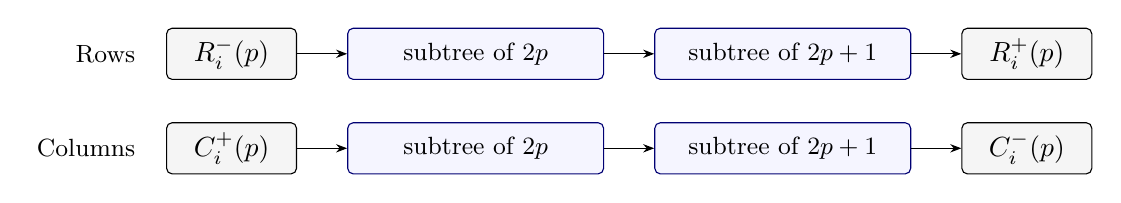
\begin{tikzpicture}[x=1cm,y=1cm,
 parent/.style={draw,rounded corners=2pt,minimum width=1.65cm,minimum height=.65cm,fill=black!4},
 child/.style={draw=blue!45!black,rounded corners=2pt,minimum width=3.25cm,minimum height=.65cm,fill=blue!4,font=\small},
 >={Stealth[length=4pt]}]
\node[anchor=east,font=\small] at (-.1,1.2) {Rows};
\node[parent] (rm) at (1,1.2) {$R_i^-(p)$};
\node[child] (r0) at (4.1,1.2) {subtree of $2p$};
\node[child] (r1) at (8.0,1.2) {subtree of $2p+1$};
\node[parent] (rp) at (11.1,1.2) {$R_i^+(p)$};
\draw[->] (rm.east)--(r0.west);
\draw[->] (r0.east)--(r1.west);
\draw[->] (r1.east)--(rp.west);
\node[anchor=east,font=\small] at (-.1,0) {Columns};
\node[parent] (cp) at (1,0) {$C_i^+(p)$};
\node[child] (c0) at (4.1,0) {subtree of $2p$};
\node[child] (c1) at (8.0,0) {subtree of $2p+1$};
\node[parent] (cm) at (11.1,0) {$C_i^-(p)$};
\draw[->] (cp.east)--(c0.west);
\draw[->] (c0.east)--(c1.west);
\draw[->] (c1.east)--(cm.west);
\end{tikzpicture}
\caption{The two orders at an internal node $(i,p)$, where $i<h$.
Each blue box contains the entire corresponding subtree on that axis.
At a leaf, the minus and plus names denote the same single position.
The reversed parent signs give the four comparisons in
\eqref{eq:tree-orders}.}
\label{fig:tree-orders}
\end{figure}



Two elementary restrictions explain the body roles we use. For binary
values $a,b$,
\[
 \begin{pmatrix}1&a\\1&b\end{pmatrix}\ne P
       \quad\Longleftrightarrow\quad b\le a,
 \qquad
 \begin{pmatrix}a&b\\1&1\end{pmatrix}\ne P
       \quad\Longleftrightarrow\quad a\le b.
\]
We will supply the fixed ones with a dummy column in the first array
and a dummy row in the second. The first restriction passes a value
between consecutive row levels; the second passes it between
consecutive column levels. In either inequality, knowing that the
smaller entry is $1$ forces the larger entry to be $1$, while knowing
that the larger entry is $0$ forces the smaller entry to be $0$.

To specify which rows and columns have these roles, define a set $T$
of $6h$ indices, called \emph{modes}. Each mode specifies two row sets
and two column sets as follows, where $1\le i\le h$ and
$d\in\{0,1\}$:
\begin{equation}
 \begin{array}{c|cc|cc}
 t&\mathsf R_1(t)&\mathsf R_2(t)&\mathsf C_1(t)&\mathsf C_2(t)\\ \hline
 V_i^+&R_i^+&R_{i-1}^+&C_*&C_{i-1}^+\\
 V_i^-&R_{i-1}^-&R_i^-&C_*&C_{i-1}^-\\
 W_{i,d}^+&R_{i,d}^+&R_*&C_{i-1}^+&C_{i,d}^+\\
 W_{i,d}^-&R_{i,d}^-&R_*&C_{i,d}^-&C_{i-1}^-
 \end{array}
 \label{eq:body-modes}
\end{equation}
The $V$ modes pair consecutive row levels with a dummy column; the
$W$ modes pair consecutive column levels with a dummy row and fix the
child parity.
For each $t$, its two row sets are disjoint and its two column sets
are disjoint.  An ordered body in mode $t$ uses rows $r_1<r_2$ with
$r_j\in\mathsf R_j(t)$ and columns $c_1<c_2$ with
$c_j\in\mathsf C_j(t)$.  The order conditions remain part of this
definition; the two role sets need not precede one another as entire
sets.

Fix the order of modes by increasing $i$, with the six modes at depth
$i$ ordered as
\[
 V_i^+,\quad V_i^-,\quad W_{i,0}^+,\quad W_{i,1}^+,\quad
 W_{i,0}^-,\quad W_{i,1}^-.
\]
Before all variable and dummy positions on each axis, place an anchor
block for each mode, in this mode order.  The row block of mode $t$
has successive groups $\widehat R_t(u)$, $1\le u\le s$, and its
column block has successive groups $\widehat C_t(v)$, $1\le v\le s$.
Each group has size $m$.
Positions in these groups are \emph{anchor positions}; the variable
and dummy positions are \emph{non-anchor positions}.

There are $6hs$ anchor groups on each axis.  The variable positions
form $2h+1$ disjoint sets of size $m$: two signs at each depth below
$h$, and one set of leaves.  Including the dummy block, the total
number of positions on either axis is therefore
\begin{equation}
 n=d_hm,\qquad d_h=6hs+2h+2=386h+2.
 \label{eq:matrix-size}
\end{equation}
Identify each resulting ordered axis with $[n]$.

\subsection{All binary entries}

Define $A_h\in\{0,1\}^{[n]\times[n]}$ by the following rules.
They assign every entry, with no extra labels attached to the matrix.
\begin{enumerate}
 \item Between anchor groups $\widehat R_t(u)$ and
 $\widehat C_{t'}(v)$, put $S(u,v)$ if $t=t'$ and put $0$ otherwise.

 \item For a non-anchor row $r$, its values against the $s$ anchor
 column groups of mode $t$ are $e_j^{\mathsf T}$ if
 $r\in\mathsf R_j(t)$, and the zero word if it belongs to neither
 row set.  Similarly, for a non-anchor column $c$, its values against
 the anchor row groups of mode $t$ are $e_j$ if
 $c\in\mathsf C_j(t)$, and zero if it belongs to neither column set.
 The disjointness of the two role sets makes both instructions
 unambiguous.

 \item Between non-anchor positions, put $1$ whenever the row or
 column is dummy.  Between variable positions, use the following
 table, putting $0$ in every case absent from the table:
 \begin{equation}
  \begin{array}{ccc|c}
   \text{row block}&\text{column block}&\text{depth range}&A_h\\ \hline
   R_i^+(p)&C_i^+(q)&0\le i\le h&\mathbf1[p\le q]\\
   R_i^-(p)&C_i^-(q)&0\le i<h&\mathbf1[p<q]\\
   R_i^+(p)&C_{i-1}^+(q)&1\le i\le h&\mathbf1[\pi(p)\le q]\\
   R_i^-(p)&C_{i-1}^-(q)&1\le i\le h&\mathbf1[\pi(p)<q]
  \end{array}
  \label{eq:variable-entries}
 \end{equation}
\end{enumerate}
Every displayed value is constant on the corresponding pair of blocks.
The first two lines of \eqref{eq:variable-entries} have disjoint ranges
of blocks because the second excludes the shared leaves.  In the last
two lines the column depth is below $h$, so their two column signs
remain distinct even when the row is a shared leaf.  Thus the table
has no conflicting assignments.  In particular, the entry between
leaf blocks of indices $p,q$ is always $\mathbf1[p\le q]$.

\section{Distance under arbitrary binary changes}
\label{sec:distance}

We first prove that fewer than $m^2$ binary changes cannot eliminate
all copies of $H$. We choose one path through the tree on each axis,
with the same node indices, so that its root entries and sampled anchor
and dummy incidences are unchanged. All other entries between variable
positions may change freely. If the edited matrix were $H$-free, its
mode restrictions would then force opposite values on the shared leaf
entry.

\begin{proposition}\label{prop:distance}
Let $h\geq 1$, let $m=2^h$, and let $A=A_h$ be the matrix constructed
above, of order $n=d_hm$, where $d_h=386h+2$.  Every $H$-free binary
$n\times n$ matrix differs from $A$ in at least $m^2$ entries.
Consequently $A$ is $d_h^{-2}$-far from being $H$-free.
\end{proposition}

\begin{proof}
Fix an arbitrary binary matrix $B$ differing from $A$ on a set $E$ of
$M<m^2$ cells.  We will find a copy of $H$ in $B$.

\paragraph{Choosing positions while avoiding the relevant changes.}
On each axis, partition the positions into the anchor groups, the dummy
group, the variable classes at levels $0,\ldots,h-1$ for each sign, and
the one shared leaf class.  All these classes have size $m$.  In
particular, the leaf class occurs once in this partition, despite its
two sign names.

Choose $z$ uniformly from $\{0,\ldots,m-1\}$ and put
\[
 a_i=\left\lfloor\frac{z}{2^{h-i}}\right\rfloor
 \qquad(0\leq i\leq h).
\]
Thus $a_i$ indexes the ancestor at level $i$ of leaf $z$, and
$\lfloor a_i/2\rfloor=a_{i-1}$.  Choose positions
\[
 x_i^\sigma\in R_i^\sigma(a_i),\qquad
 y_i^\sigma\in C_i^\sigma(a_i)
 \qquad(\sigma\in\{+,-\}),
\]
uniformly within their blocks, using a single shared choice on each axis
at the leaf:
$x_h^+=x_h^-$ and $y_h^+=y_h^-$.  Also choose one uniform position from
every anchor group and from each dummy group; denote the dummy choices
by $x_*$ and $y_*$.  Conditional on $z$, all choices in distinct groups
are independent, including choices on opposite axes.

Each variable choice is uniform on its size-$m$ class.  Indeed, a fixed
node at depth $i$ is selected with probability $2^{-i}$, and its block
has size $m/2^i$, so each position in that class is selected with
probability $1/m$.  An anchor or dummy choice is independent of every
choice on the opposite axis.  The root choices are also independent
uniform choices in their fixed size-$m$ blocks.  It follows that, for
every cell $(r,c)$ having at least one anchor or dummy position, or
having both positions at the root level,
\[
 \Pr(r\text{ and }c\text{ are selected})=\frac1{m^2}.
\]
There is only one choice in each size-$m$ class, so each cell occurs in
this calculation once.  Summing over the changed cells of these types
gives
\begin{equation}\label{eq:cellwise-bound}
 \Pr\bigl(\text{some selected cell of these types belongs to }E\bigr)
 \leq\frac{|E|}{m^2}<1.
\end{equation}
Fix a selection avoiding all such changes.  Thus all selected anchor
and dummy incidences, and the selected root entries, agree in $A$ and
$B$.  Changes at every other cell remain unrestricted.

\paragraph{What a mode forbids.}
For each mode $t$, its selected anchor positions form the matrix $S$
in $B$.  They precede all selected non-anchor positions, and their
entries to the selected positions in $\mathsf R_j(t)$ and
$\mathsf C_j(t)$ are the prescribed vectors $e_j$.
Therefore any ordered pair of selected rows in
$\mathsf R_1(t),\mathsf R_2(t)$ and ordered pair of selected columns in
$\mathsf C_1(t),\mathsf C_2(t)$ whose entries in $B$ form
\[
 P=\begin{pmatrix}1&0\\1&1\end{pmatrix}
\]
complete these anchors to a copy of $H$.
Suppose, for a contradiction, that $B$ is $H$-free.  Then this body
matrix cannot occur for any mode.

\paragraph{Propagating the root values.}
The unchanged root entries give
\begin{equation}\label{eq:root-bits}
 B(x_0^+,y_0^+)=1,\qquad B(x_0^-,y_0^-)=0.
\end{equation}
We claim that the same two equalities hold at every level:
\begin{equation}\label{eq:propagation-bits}
 B(x_i^+,y_i^+)=1,\qquad B(x_i^-,y_i^-)=0
 \qquad(0\leq i\leq h).
\end{equation}
Assume they hold at level $i-1$, where $1\leq i\leq h$.
For $V_i^+$ use rows $x_i^+,x_{i-1}^+$ and columns
$y_*,y_{i-1}^+$.  For $V_i^-$ use rows
$x_{i-1}^-,x_i^-$ and columns $y_*,y_{i-1}^-$.  These are in their
designated sets and in the required order because the chosen nodes are
parent and child.  Their body matrices in $B$ are respectively
\[
 \begin{pmatrix}
  1&B(x_i^+,y_{i-1}^+)\\1&1
 \end{pmatrix},\qquad
 \begin{pmatrix}
  1&0\\1&B(x_i^-,y_{i-1}^-)
 \end{pmatrix}.
\]
The dummy incidences supply the left column of ones.  Avoiding $P$
forces
\[
 B(x_i^+,y_{i-1}^+)=1,\qquad
 B(x_i^-,y_{i-1}^-)=0.
\]
To carry these values to level-$i$ columns, put $d=a_i\bmod 2$.
For $W_{i,d}^+$ use rows $x_i^+,x_*$ and columns
$y_{i-1}^+,y_i^+$; for $W_{i,d}^-$ use rows $x_i^-,x_*$ and columns
$y_i^-,y_{i-1}^-$.  Again these positions have the required order
and membership.  The resulting matrices are
\[
 \begin{pmatrix}
  1&B(x_i^+,y_i^+)\\1&1
 \end{pmatrix},\qquad
 \begin{pmatrix}
  B(x_i^-,y_i^-)&0\\1&1
 \end{pmatrix}.
\]
Here the bottom rows are unchanged dummy incidences.  Avoiding $P$
forces exactly \eqref{eq:propagation-bits} at level $i$, completing
the induction.

At level $h$, the two asserted values in
\eqref{eq:propagation-bits} concern the same cell, since the leaf
positions were shared.  This contradiction proves that $B$ contains
$H$.  Since every matrix with fewer than $m^2$ changes has this
property and $n=d_hm$, the normalized distance is at least
$m^2/n^2=d_h^{-2}$.
\end{proof}

\section{Copies are confined to the leaf diagonal}
\label{sec:copies}

The distance proof used the prescribed anchor representatives. To
bound the number of copies in the unedited matrix $A_h$, we must now
locate every possible copy. Its $64\times64$ prefix will lie in the
anchor groups of a single mode, and its two remaining rows and columns
will then belong to that mode's designated sets.

\subsection{The anchor and the non-anchor traces}

The anchor matrix $S$ has two complementary features. Its lower-right
corner contains every binary word of length five. We will show that
non-anchor rows cannot realize all these words on five non-anchor
columns. This will force more than $32$ positions on at least one axis of any copy to be anchors.
The dense first $32$ rows and columns, contrasted with the sparse
variable-to-anchor incidences and the zero entries between different
modes, will then force the whole copy into one mode.

\begin{lemma}[Properties of the anchor]
\label{lem:anchor-properties}
The rows of $S$ are pairwise distinct, as are its columns. Every column
has at most one zero in the first $32$ rows, and every row has at most
one zero in the first $32$ columns. Each row has at least $58$ ones and
each column has at least $48$ ones. Finally, the restrictions of rows
$33,\ldots,64$ to columns $60,\ldots,64$ are the $32$ distinct binary
words of length five.
\end{lemma}

\begin{proof}
The replacement in the definition of $S$ does not meet the first
$32$ rows or the first $59$ columns. In the first $59$ columns, each
of rows $1,\ldots,59$ has its own distinguishing zero, while rows
$60,\ldots,64$ consist entirely of ones. The latter five rows are
distinct in the replacement block. Thus the rows are distinct, and
each has at least $58$ ones.

Each of the first $59$ columns has exactly one zero, in its own row.
The last five columns are distinct because they are distinct
coordinates on the list of all binary words of length five. Each has
exactly $16$ zeros, all in the replacement block, so it also differs
from every earlier column and has $48$ ones. The remaining assertions
follow directly from the location and definition of that block.
\end{proof}

\begin{lemma}[Incidence with the modes]
\label{lem:mode-incidences}
A variable position on either axis belongs to designated sets of at
most four modes. Consequently, against any collection containing at
most one representative of each anchor group on the opposite axis,
a variable position has at most four entries equal to one.
\end{lemma}

\begin{proof}
Consider a non-leaf row in $R_i^\sigma(p)$. The only possible modes
are $V_i^\sigma$, $V_{i+1}^\sigma$, and $W_{i,d}^\sigma$, where
$d=p\bmod2$; modes whose level is outside $1,\ldots,h$ are omitted.
A leaf row belongs to $V_h^+$, $V_h^-$, and the two modes
$W_{h,d}^+$, $W_{h,d}^-$. There are at most four in either case.

For a non-leaf column in $C_i^\sigma(p)$, the possible modes are
$V_{i+1}^\sigma$, $W_{i+1,0}^\sigma$,
$W_{i+1,1}^\sigma$, and $W_{i,d}^\sigma$, again omitting undefined
levels. A leaf column belongs only to $W_{h,d}^+$ and $W_{h,d}^-$.
For each participating mode, the entries to its anchor groups form
one unit vector. This proves the last assertion as well.
\end{proof}

A set of columns is \emph{shattered} by a set of rows if the
restrictions of those rows to the columns include every binary word
of the corresponding length.

\begin{lemma}[No five non-anchor columns are shattered]
\label{lem:nonanchor-traces}
For any five distinct non-anchor columns of $A_h$, the non-anchor
rows do not realize all $32$ binary words on those columns.
\end{lemma}

\begin{proof}
If one of the five columns is a dummy column, its entry is one in
every non-anchor row, so the conclusion is immediate. Otherwise all
five columns are variable. Partition them according to their classes
$C_i^\sigma$, counting the common leaf class only once.

Within each such class, order the selected columns by node index
(and arbitrarily within a node block). The entry rules for $A_h$
show that the ones of a variable row form a suffix in each class in
which that row is nonzero. A non-leaf row is nonzero in at most two
classes: its own level and sign, and the preceding level with the
same sign. A leaf row is nonzero in at most three classes: the common
leaf class and the two signs at level $h-1$.

A class containing $a$ selected columns has at most $a$ distinct
nonempty suffixes. Across all classes there are therefore at most
five such suffixes. The trace of a variable row is a union of at most
three of them, giving at most
\[
   \sum_{j=0}^3\binom{5}{j}=26
\]
possible traces. The dummy rows contribute at most one additional
trace. Thus at most $27<32$ words occur.
\end{proof}

\subsection{Every anchor copy uses one mode}

\begin{lemma}[Anchor rigidity]
\label{lem:anchor-rigidity}
Every ordered copy of $S$ in $A_h$ uses the row and column anchor
groups of a single mode $t$. On each axis it uses exactly one position
from each of that mode's $64$ groups, in their prescribed order.
\end{lemma}

\begin{proof}
Fix an ordered copy of $S$. Two positions in a single anchor group
have identical entries throughout $A_h$. By
Lemma~\ref{lem:anchor-properties}, the copy therefore uses at most
one position from any one anchor group. The same reasoning shows
that it uses at most one dummy position on each axis.

Suppose that at most $32$ selected rows and at most $32$ selected
columns are anchors. Since all anchors precede all non-anchor
positions, the last $32$ selected rows and the last five selected
columns are non-anchor positions. Their entries give all $32$ binary
words by Lemma~\ref{lem:anchor-properties}, contrary to
Lemma~\ref{lem:nonanchor-traces}. Hence more than $32$ selected
positions are anchors on at least one axis.

Assume first that more than $32$ selected rows are anchors. In
particular the first $32$ selected rows are anchors. No selected
column can be variable: Lemma~\ref{lem:mode-incidences} would give
at most four ones in these rows, whereas each column of $S$ has at
least $31$ ones in its first $32$ rows. There are consequently at
least $63$ selected anchor columns, since at most one selected
column is dummy.

Any two selected anchor columns have a common one among the first
$32$ selected rows: each has at most one zero there. They must
therefore belong to the same mode, because entries between anchor
groups of different modes are zero. Write $t$ for this common mode.
Every selected anchor row also belongs to $t$. Indeed an anchor row
of another mode would be zero on the at least $63$ selected anchor
columns and would have at most one one in the entire copy,
contradicting Lemma~\ref{lem:anchor-properties}.

A selected dummy column is now impossible: its entries to the
selected anchor rows of mode $t$ contain at most one one, because
its entries to that mode form either a unit vector or the zero
vector. This again contradicts the density of the first $32$ rows
of $S$. Thus all selected columns are anchors of mode $t$. Any
non-anchor row has at most one one against those columns, so every
selected row must also be an anchor of $t$.

If instead more than $32$ selected columns are anchors, the same
argument applies with the axes interchanged. All properties used
after the preceding case distinction are symmetric in the axes:
entries between different anchor modes are zero, the first $32$
rows and columns of $S$ each contain at most one zero in the relevant
restriction, all its rows and columns have more than one one, and
Lemma~\ref{lem:mode-incidences} holds on both axes.

There are $64$ selected positions on each axis and only $64$ anchor
groups in mode $t$. No group is repeated, so every group is used.
Their order in the construction is their order in the copy.
\end{proof}

\begin{corollary}[The two body roles]
\label{cor:body-roles}
In every ordered copy of $H$ in $A_h$, the first $64$ rows and
columns are anchor representatives of one mode $t$. Its two body
rows belong respectively to $\mathsf R_1(t),\mathsf R_2(t)$, and its
two body columns belong respectively to
$\mathsf C_1(t),\mathsf C_2(t)$.
\end{corollary}

\begin{proof}
Apply Lemma~\ref{lem:anchor-rigidity} to the copy's prefix $S$.
The two body rows must have entries $e_1^{\mathsf T}$ and
$e_2^{\mathsf T}$ against these anchor columns. An anchor row of
another mode gives the zero vector; an anchor row of mode $t$ gives
a row of $S$, which has more than one one. Thus neither body row is
an anchor. By the definition of the entries between non-anchor
positions and anchor groups, the vector $e_j^{\mathsf T}$ occurs
exactly on $\mathsf R_j(t)$, for $j=1,2$. The two designated sets are
disjoint. The column argument is identical.
\end{proof}

\subsection{Every copy uses a diagonal leaf cell}
\label{subsec:copy-count}

The body restrictions from Corollary~\ref{cor:body-roles} leave only one
possible source of copies: the two signs share the same positions at the
leaves.  We now locate that source at a fixed entry of the pattern.

\begin{proposition}\label{prop:copy-count}
For every integer $h\geq 1$, every ordered copy of $H$ in $A_h$ maps the
pattern entry $(s+1,s+1)$ into
\[
 \mathcal L_h
 =\bigcup_{p=0}^{m-1} R_h^+(p)\times C_h^+(p).
\]
In particular, $|\mathcal L_h|=m$ and
\begin{equation}\label{eq:copy-bound}
 N_H(A_h)\leq m n^{2k-2},
 \qquad
 \frac{N_H(A_h)}{n^{2k}}
 \leq \frac{2^{-h}}{d_h^2}.
\end{equation}
\end{proposition}

\begin{proof}
By Corollary~\ref{cor:body-roles}, the last two rows and columns of an
$H$-copy lie in the prescribed body sets of a single mode.  Their entries
must form
\[
 P=\begin{pmatrix}1&0\\1&1\end{pmatrix}.
\]
We check the four kinds of modes, using the order equivalences
\eqref{eq:tree-orders} and the entry rules \eqref{eq:variable-entries}.
Write $\pi(p)=\lfloor p/2\rfloor$ for
the parent index of a node.

In mode $V_i^+$, let $p$ be the child-level row index, $a$ the parent-level
row index, and $b$ the parent-level column index.  The order of the two
rows gives $\pi(p)\leq a$.  The bottom-right entry of $P$ gives $a\leq b$.
Consequently $\pi(p)\leq b$, so the top-right entry is $1$, a
contradiction.

In mode $V_i^-$, use the same names for the node indices at the same
levels.  The row order gives $\pi(p)\geq a$, while the top-right entry
$0$ gives $a\geq b$.  Thus $\pi(p)\geq b$, and the bottom-right entry is
$0$, again a contradiction.

In mode $W_{i,d}^+$, let $p,q$ be the child-level row and column indices,
and let $b$ be the parent-level column index.  The column order gives
$b\leq\pi(q)$, and the top-left entry $1$ gives $\pi(p)\leq b$.
Since $p\equiv q\equiv d\pmod 2$, it follows that $p\leq q$.  The
top-right entry is therefore $1$, contrary to $P$.

Finally, in mode $W_{i,d}^-$, the column order gives $\pi(q)\leq b$,
and the top-right entry $0$ gives $\pi(p)\geq b$.  The common parity
implies $p\geq q$.  If $i<h$, the top-left entry is
$\mathbf 1[p<q]=0$, which is impossible.  If $i=h$, that entry is instead
$\mathbf 1[p\leq q]$, because the leaf blocks are shared.  It can be $1$
only when $p=q$.  This places the top-left entry of the body, namely
$(s+1,s+1)$ in $H$, in $\mathcal L_h$.

Each leaf block has size $m/2^h=1$, so $\mathcal L_h$ contains exactly
$m$ cells.  For each such cell, fix the images of row $s+1$ and column
$s+1$ of $H$.  There are at most $n^{k-1}$ choices for the other row
indices and at most $n^{k-1}$ choices for the other column indices;
requiring increasing orders and the prescribed entries can only reduce
these numbers.  This proves the first inequality in
\eqref{eq:copy-bound}.  Since $n=d_hm$ and $m=2^h$, division by $n^{2k}$
gives the second.
\end{proof}


\begin{remark}\label{rem:hitting-not-repair}
Changing the $m$ entries of $\mathcal L_h$ from $1$ to $0$ destroys every
original copy, but creates new ones. Indeed, fix a leaf index $p$ and put
$d=p\bmod 2$. In mode $W_{h,d}^+$, choose the leaf row in $R_h^+(p)$
and any dummy row. Choose, in this order, a column in
$C_{h-1}^+(\pi(p))$ and the leaf column in $C_h^+(p)$.
These rows and columns have the required order. Their body is now
\[
 \begin{pmatrix}1&0\\1&1\end{pmatrix}:
\]
the upper-left entry is the unchanged parent--child entry, the
upper-right entry is the changed leaf diagonal, and the lower entries
are dummy incidences. Choosing one position from every anchor group
of this mode completes a new copy of $H$, since all anchor entries and
signatures are unchanged. Thus an original-copy hitting set need not
provide an $H$-free repair.
\end{remark}

\section{Proof of the main theorem}
\label{sec:conclusion}

The construction uses the same $66\times 66$ pattern $H$ at every depth.
The two preceding estimates now give the required counterexamples.

\begin{proof}[Proof of Theorem~\ref{thm:main}]
For each integer $h\geq1$, set
\[
 \epsilon_h=d_h^{-2}=(386h+2)^{-2},
 \qquad n_h=d_h2^h.
\]
Proposition~\ref{prop:distance} shows that every $H$-free binary matrix
differs from $A_h$ in at least $m^2=\epsilon_h n_h^2$ entries.
Proposition~\ref{prop:copy-count} gives
\[
 \frac{N_H(A_h)}{n_h^{132}}
 \leq \epsilon_h2^{-h}.
\]
These statements prove the asserted construction sequence.

Now fix arbitrary real numbers $c,C>0$.  As $h$ tends to infinity,
\[
 \frac{N_H(A_h)}{\epsilon_h^C n_h^{132}}
 \leq (386h+2)^{2C-2}2^{-h}
 \longrightarrow 0.
\]
Choose an integer $h$ for which the right-hand side is less than $c$.
Then $0<\epsilon_h<1$, the matrix $A_h$ is $\epsilon_h$-far from being
$H$-free, and
$N_H(A_h)<c\epsilon_h^C n_h^{132}$, as required.
\end{proof}

\begin{corollary}[Canonical row--column sampling]
\label{cor:canonical-testing}
Fix $h\ge1$ and an integer $0\le q\le n_h$. Consider a tester that
chooses a uniformly random $q$-element row set $R\subseteq[n_h]$ and,
independently, a uniformly random $q$-element column set
$C\subseteq[n_h]$. It rejects only if the induced submatrix $A_h[R,C]$,
with the inherited orders, contains an ordered copy of $H$. Then
\[
 \Pr(\text{reject on }A_h)\le\epsilon_h2^{-h}q^2,
\]
and the rejection probability is zero when $q<66$. For every fixed
$\rho\in(0,1]$, rejection probability at least $\rho$ requires
\[
 q\ge\sqrt{\rho}\,\epsilon_h^{-1/2}2^{h/2},
\]
hence $q\ge\exp(\Omega(\epsilon_h^{-1/2}))$ along the sequence
$\epsilon_h$ as $h\to\infty$. Here $q$ is the sample size on each axis;
the induced submatrix has $q^2$ entries.
\end{corollary}

\begin{proof}
By Proposition~\ref{prop:copy-count}, every copy of $H$ in $A_h$ uses a
cell of $\mathcal L_h$, and $|\mathcal L_h|=2^h$. For each fixed cell
$(r,c)$, independence gives
$\Pr((r,c)\in R\times C)=(q/n_h)^2$. Rejection implies that
$R\times C$ meets $\mathcal L_h$, so the union bound gives
\[
 \Pr(\text{reject on }A_h)
 \le 2^h(q/n_h)^2=\epsilon_h2^{-h}q^2.
\]
If $q<66$, the sampled submatrix cannot contain $H$. Rearranging the
probability bound gives the necessary sample size, and
$\epsilon_h^{-1/2}=386h+2$ gives its exponential growth along the
stated sequence.
\end{proof}

\bibliographystyle{alpha}
\bibliography{references}
\end{document}
